\documentclass{beamer}
\mode<presentation>
{
  \usetheme{default}      % or try Darmstadt, Madrid, Warsaw, ...
  \usecolortheme{default} % or try albatross, beaver, crane, ...
  \usefonttheme{default}  % or try serif, structurebold, ...
  \setbeamertemplate{navigation symbols}{}
  \setbeamertemplate{caption}[numbered]
} 

\usepackage[slovene]{babel}
\usepackage{graphicx, amsmath, listings, amssymb, commath, float}
\usepackage[utf8]{inputenc}
\usepackage[section]{placeins}

\title{Presek dveh implicitno danih ploskev}
\author[Avtorji]{Aljaž Verlič, Blažka Blatnik, Lina Lumburovska, Luka Tavčer\\
Mentor: Damir Franetič}
\date{5. junij 2017}
\begin{document}

\begin{frame}
  \titlepage
\end{frame}

\begin{frame}{Opis problema + modela (F)?}
   V $\mathbb{R}^3$ imamo podani dve poljubni implicitno podani ploskvi, opisanimi z enačbama $f_{1}(x)$ = $C_{1}$ in\\ $f_{2}(x)$ = $C_{2}$, ki ju lahko gledamo tudi kot enačbi nivojnic funkcij $f_{1}$ in $f_{2}$, presek pa je množica rešitev tega nelinearnega sistema enačb.\\
   Naša naloga je poiskati krivuljo $K$, ki predstavlja presek teh dveh ploskev.\\
   Nalogo bomo rešili na 4 načine z uporabo metod za numerično reševanje diferencialnih enačb. Uporabili bomo:
   \begin{itemize}  
   	\item Eulerjevo/Runge-Kutta s fiksno dolžino koraka
   	\item Eulerjevo/Runge-Kutta z adaptivno dolžino koraka
   \end{itemize}
\end{frame}

\begin{frame}{Opis metod?}

\end{frame}

\begin{frame}{Eulerjeva metoda + geometrična intuicija}

\end{frame}

\begin{frame}{Potrebni pogoji + J matrika}
	Potreben pogoj za delovanje metod je, da sta funkciji $f_{1}$ in $f_{2}$ parcialno odvedljivi in da ima Jacobijeva matrika parcialnih odvodov poln rang 2. Za uspešno delovanje Newtonove metode moramo poiskati Jacobijevo matriko leve strani sistema nelinearnih enačb.
	
	\begin{center}
		JG = $\begin{bmatrix}
		grad(f_{1}) \\
		grad(f_{2}) \\
		grad(\vec{v} \cdot \vec{x}) \\
		\end{bmatrix}$
		oziroma
		JG = $\begin{bmatrix}
		grad(f_{1}) \\
		grad(f_{2}) \\
		\hspace{1mm}grad(\vec{v}\hspace{0.5mm}^\intercal) \\
		\end{bmatrix}$
	\end{center}
\end{frame}

\begin{frame}{Razlaga adaptivnega koraka? (utemeljitev implementacije in zakaj je potrebna)}

\end{frame}

\begin{frame}{Koncna analiza parov ploskev za vsak primer + slike}
	Delovanje našega programa lahko preverimo s programom, ki smo ga napisali v Octave-u. Kot vhodne parametre mu podamo obe implicitno podani funkciji $f_{1}$, $f_{2}$, $C1$, $C2$, $grad(f_{1})$, $grad(f_{2})$. Določimo tudi začetni približek $x_{0}$, začetno dolžino koraka in pa parameter, ki določa metodo delovanja (Euler/Runge-Kutta).
\end{frame}

\begin{frame}{Koncna analiza parov ploskev za vsak primer + slike}
	Delovanje našega programa lahko preverimo s programom, ki smo ga napisali v Octave-u. Kot vhodne parametre mu podamo obe implicitno podani funkciji $f_{1}$, $f_{2}$, $C1$, $C2$, $grad(f_{1})$, $grad(f_{2})$. Določimo tudi začetni približek $x_{0}$, začetno dolžino koraka in pa parameter, ki določa metodo delovanja (Euler/Runge-Kutta).
\end{frame}

\begin{frame}{Primer 1}
	Začnemo z preprostim primerom sfere in ravnine, podane z enačbama:\\
	
	\begin{itemize} 
		\item $f_{1}(x,y,z)$ = $x^2 + y^2 + z^2$ = 4
		\item $f_{2}(x,y,z)$ = $3x + 2y + z$ = 1	
	\end{itemize} 
	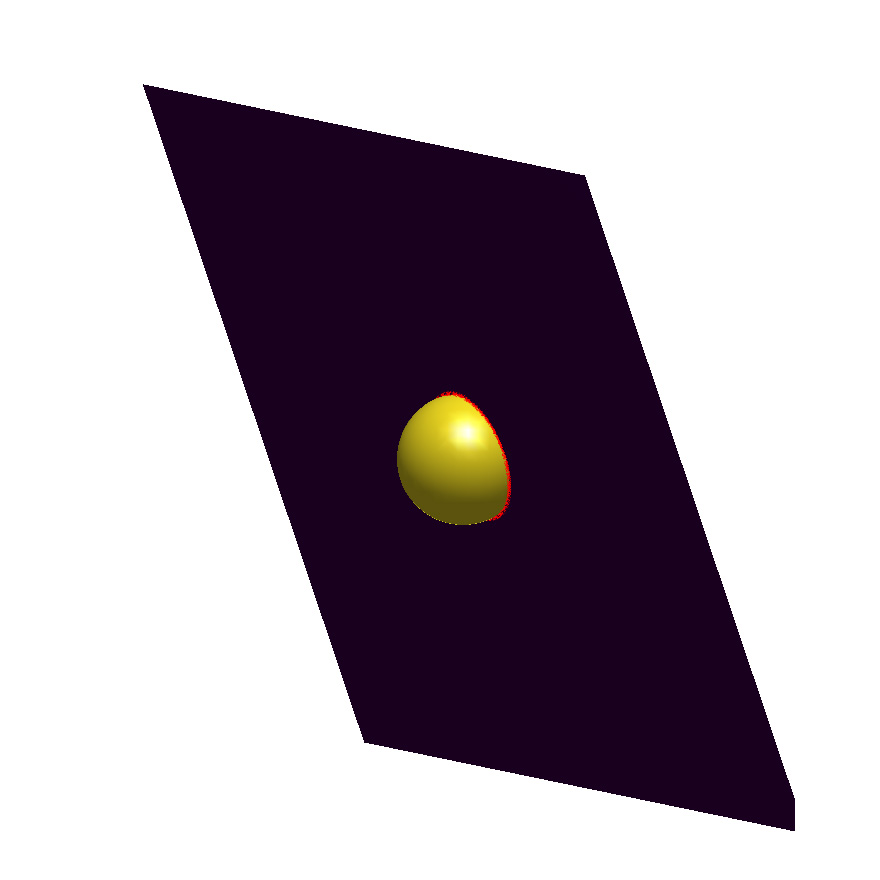
\includegraphics[scale=0.3]{primer1_1}
	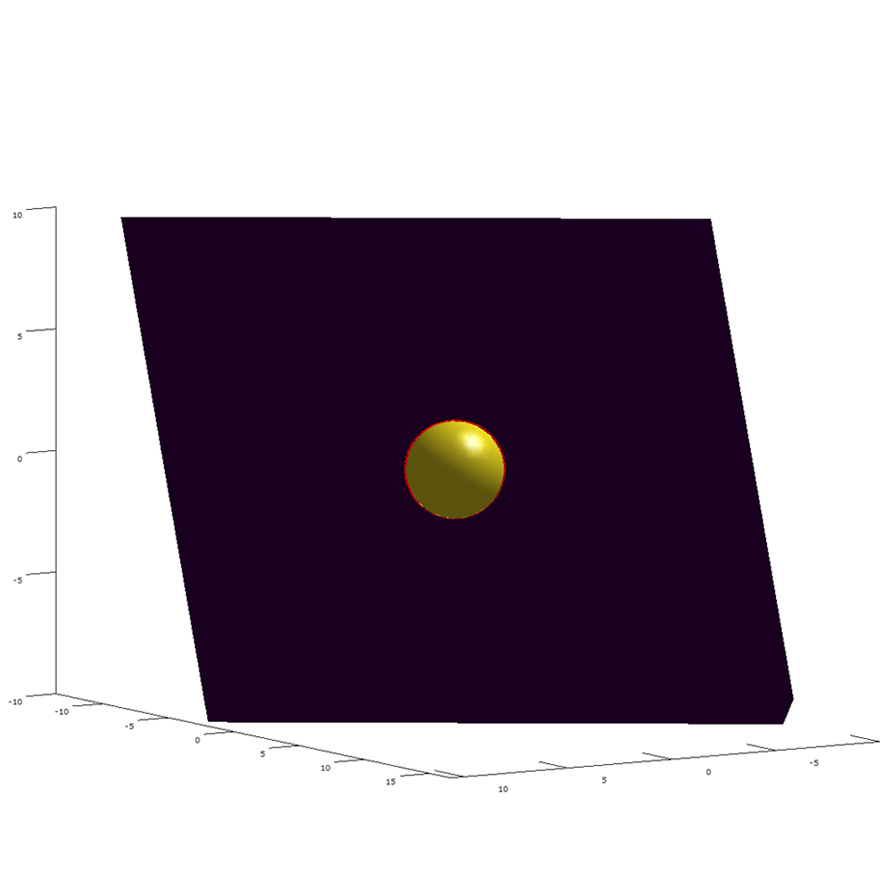
\includegraphics[scale=0.3]{primer1_2}
\end{frame}

\begin{frame}{Primer 2}
	Tudi primer sfere in valja je relativno "lep"\\
	
	\begin{itemize}  
		\item $f_{1}(x,y,z)$ = $x^2 + y^2 + z^2$ = 4
		\item $f_{2}(x,y,z)$ = $x^2 + y^2$ = 1
	\end{itemize} 
	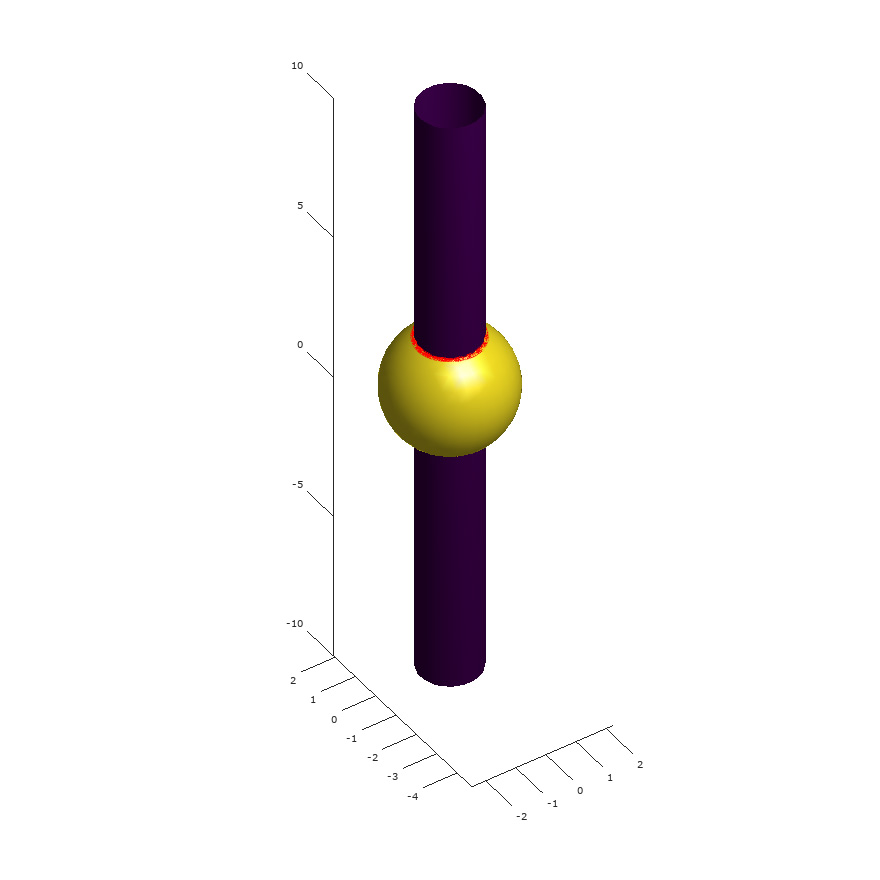
\includegraphics[scale=0.3]{primer2_1}
	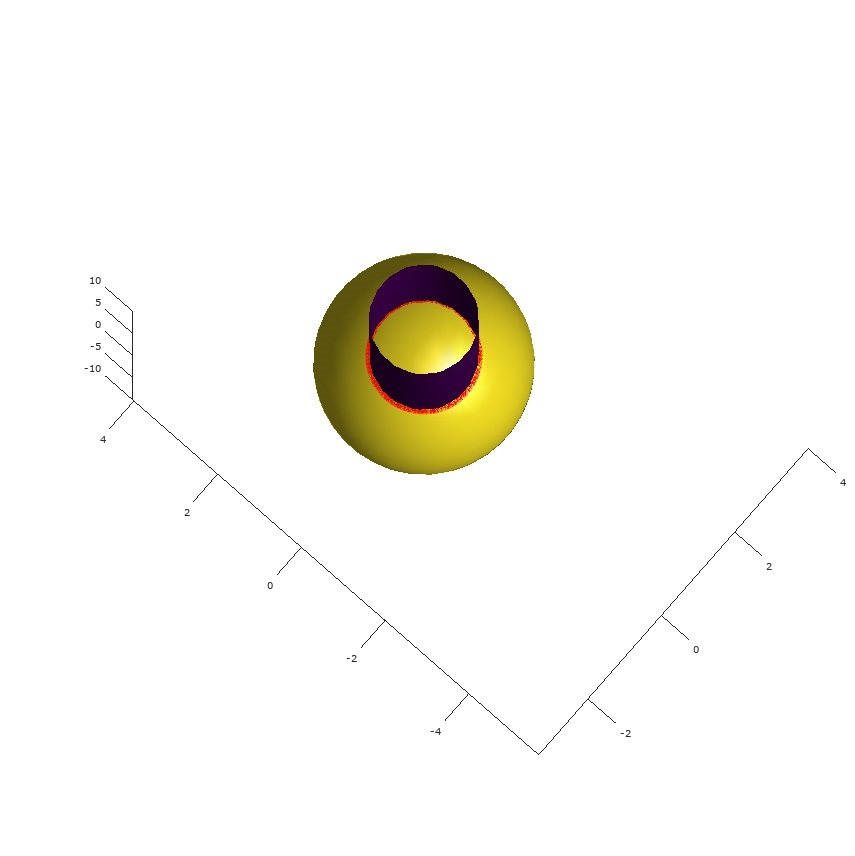
\includegraphics[scale=0.3]{primer2_2}
\end{frame}

\begin{frame}{Primer 3}
	Stvari malce otežimo s sfero in $f_{2}$
	
	\begin{itemize}  
		\item $f_{1}(x,y,z)$ = $x^2 + y^2 + z^2$ = 4
		\item $f_{2}(x,y,z)$ = $y^4 + log(x^2 + 1)z^2 - 4$ = 1
	\end{itemize} 
	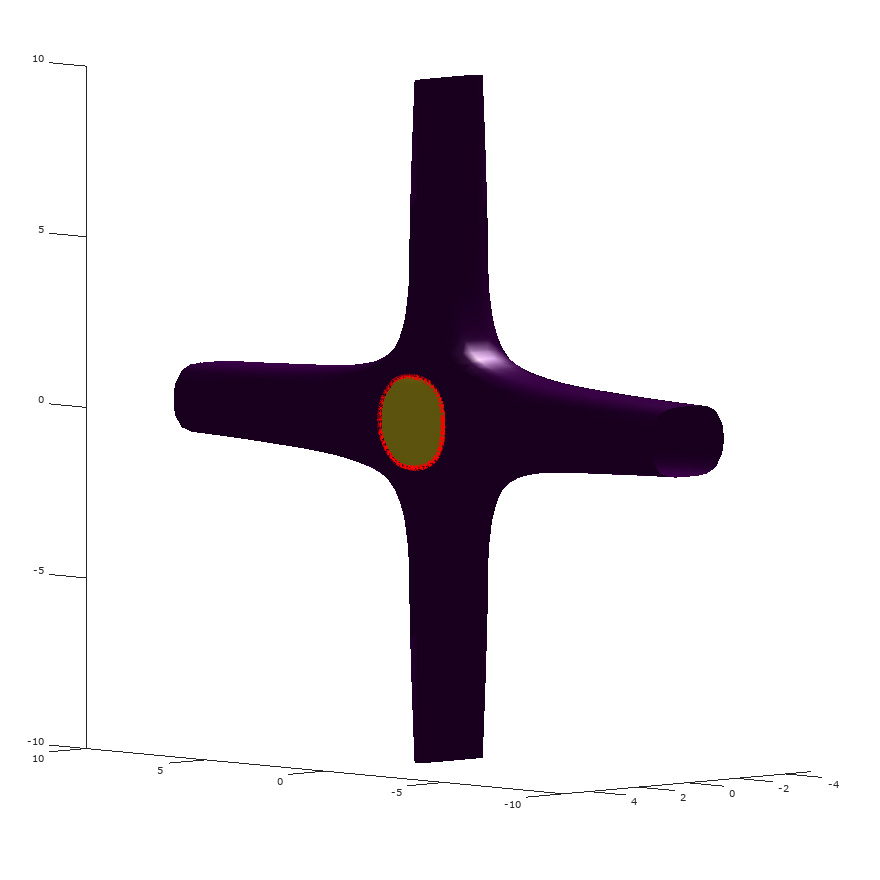
\includegraphics[scale=0.3]{primer3_1}
	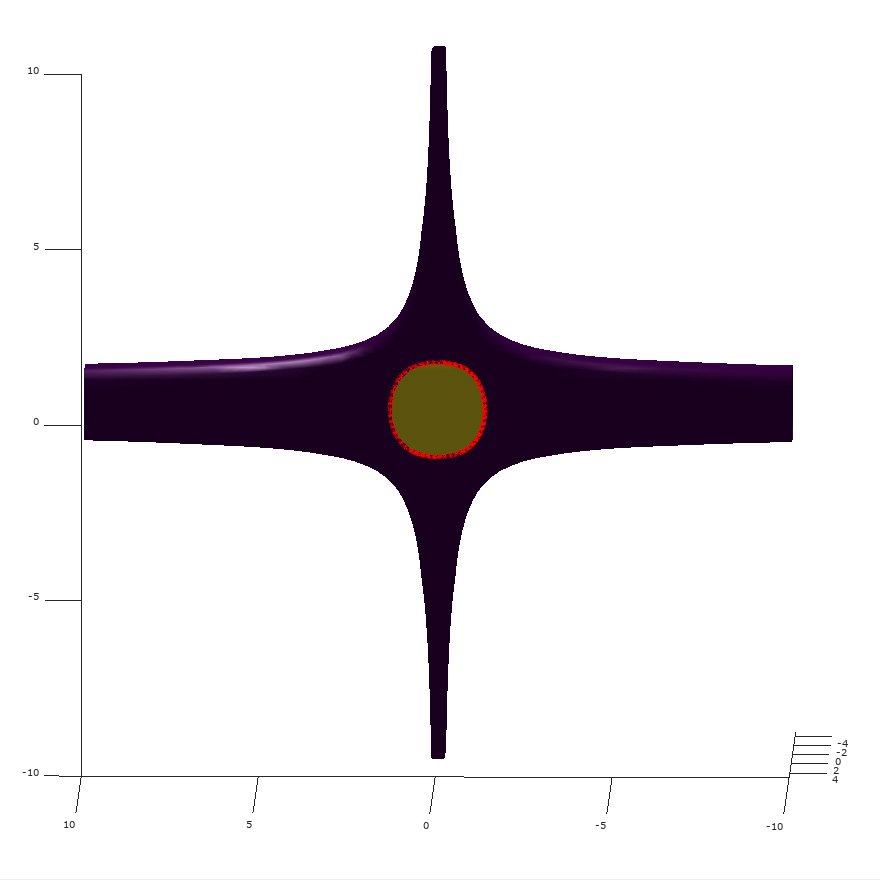
\includegraphics[scale=0.3]{primer3_2}
\end{frame}

\begin{frame}{Primer 4}
	Za konec pa\\
	
	\begin{itemize}  
		\item $f_{1}(x,y,z)$ = $x^2 + cos(y)z^2 - 12$ = 4
		\item $f_{2}(x,y,z)$ = $y^4 + log(x^2 + 1)z^2 - 4$ = 1
	\end{itemize} 
	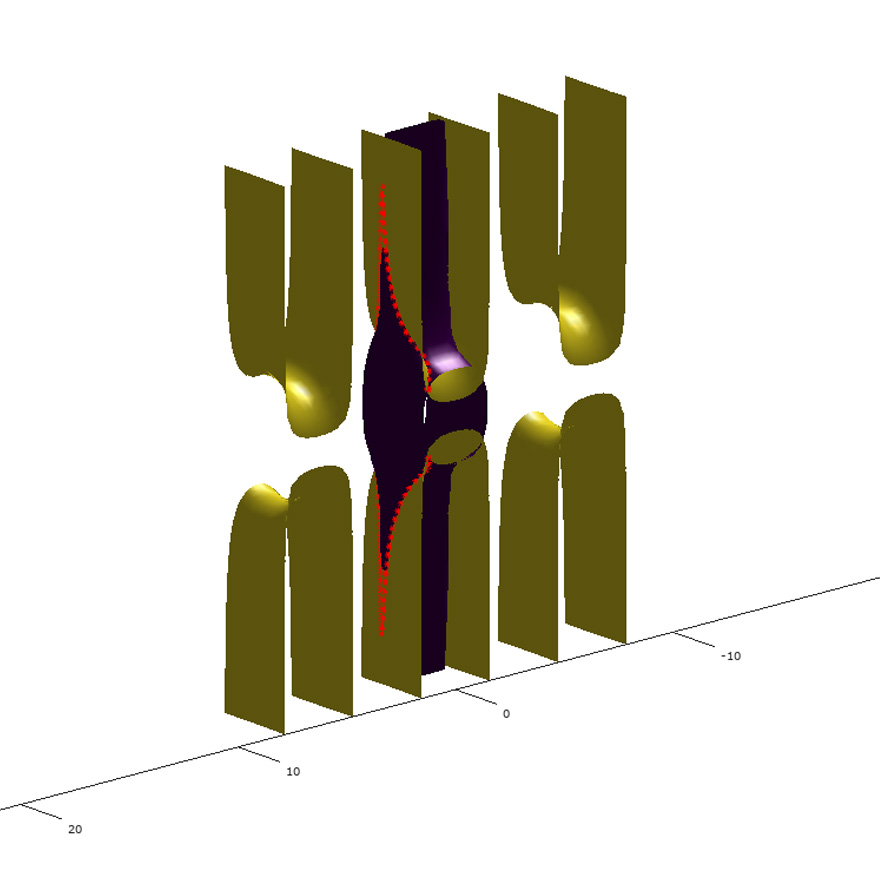
\includegraphics[scale=0.3]{primer4_1}
	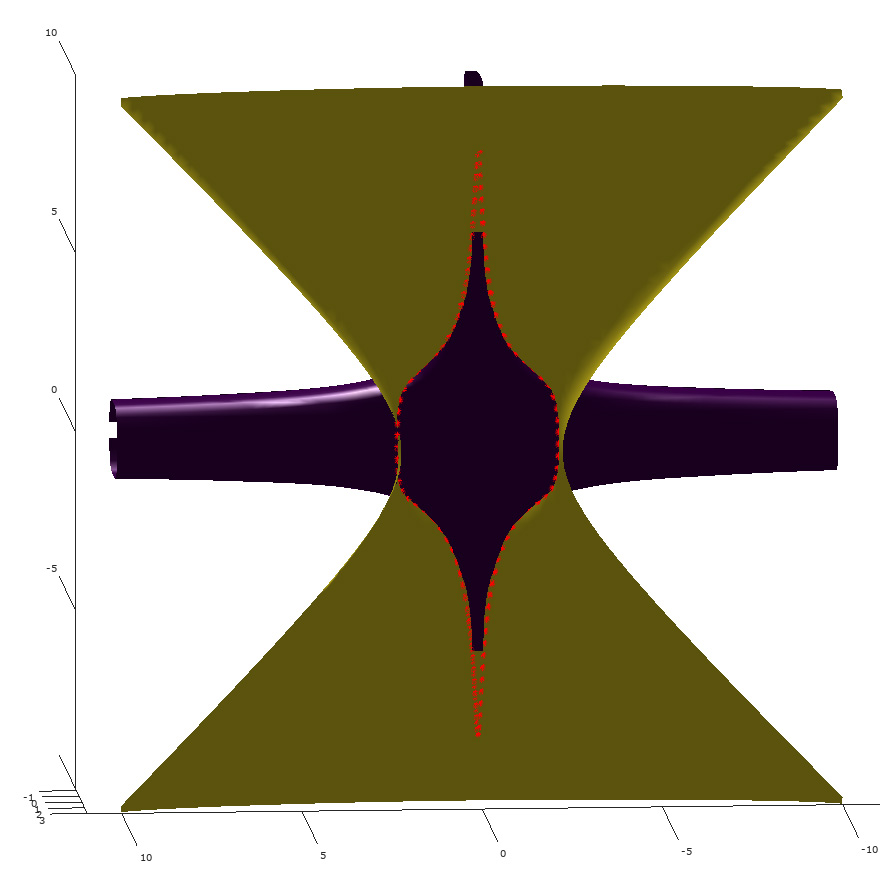
\includegraphics[scale=0.3]{primer4_2}
\end{frame}
\end{document}
